\section{问题二：共表达网络与关键化合物识别}

\subsection{问题描述}

问题二给出 \texttt{2.csv} 的化合物相关矩阵，要求建立共表达网络，并结合 \texttt{1.csv} 的化学特征与 \texttt{4.csv} 的感官标签，为每个感官维度给出 \textbf{3} 个关键化合物；同时要回答三个追问：排序是否稳定、结果是否有化学合理性、它与全局重要度排序是否一致。

这一问的输出不是一张“化合物重要性排行榜”，而是 \textbf{50} 个维度各自的 \textbf{3} 个化合物。若只按“化合物与感官维度的相关系数”排序，容易同时选中几个高度共线的同源化合物；若只按“网络中度数”排序，又会选出与感官目标无关的枢纽节点。本文把两种信息写成可加融合分，把图结构作为平滑项，并要求融合后的排序在重采样下可复核。

\subsection{模型建立}

\subsubsection{共表达图的构建}

把 \texttt{2.csv} 的 \textbf{231} 个节点剔除 \textbf{4} 个聚合列与 \textbf{1} 个热量列，保留 \textbf{226} 个候选化合物。对任意两个不同节点 $i,j$，令 $\rho_{ij}$ 为 \texttt{2.csv} 中的 Spearman 相关系数；当
\begin{equation}
\left|\rho_{ij}\right|\ge \tau
\label{eq:edge}
\end{equation}
时连一条无向边，边权取 $w_{ij}=|\rho_{ij}|$。阈值 $\tau$ 取 \textbf{0.30}。这个取值不是凭经验拍的：按 \textbf{226} 个节点共有 \textbf{25425} 个无序对、标称样本量 \textbf{250} 做 Fisher 变换，Bonferroni 校正后的单对临界值约为 \textbf{0.293754}，向上取整到 \textbf{0.30}\cite{benjamini1995}。在该阈值下，单对最大 $p$ 值仍小于校正后的显著性水平，图不会把大量噪声边纳入。

\subsubsection{直接相关得分与图平滑得分}

对化合物 $c$ 与感官维度 $d$，直接相关得分定义为
\begin{equation}
s_{\mathrm{direct}}(c,d)=\left|\mathrm{Spearman}\left(x_c,y_d\right)\right|,
\label{eq:sdirect}
\end{equation}
其中 $x_c$ 为 \texttt{1.csv} 中化合物 $c$ 的列，$y_d$ 为 \texttt{4.csv} 中第 $d$ 维标签；按列内可用样本成对计算，不插补。$s_{\mathrm{direct}}$ 衡量“这个化合物自己与感官维度有多强的关系”，但它看不见邻居。

设化合物 $c$ 的邻居集合为 $N(c)=\{j\ne c:|\rho_{cj}|\ge\tau\}$，图平滑得分定义为邻居得分的加权平均：
\begin{equation}
s_{\mathrm{graph}}(c,d)=\frac{\sum_{j\in N(c)}w_{cj}\,s_{\mathrm{direct}}(j,d)}
{\sum_{j\in N(c)}w_{cj}}.
\label{eq:sgraph}
\end{equation}
式 \eqref{eq:sgraph} 的含义是：如果一个化合物自己与感官维度的相关不算最强，但它的邻居们都与该维度强相关，那么它仍可能是该维度的关键化合物。若邻居的 $s_{\mathrm{direct}}$ 缺失，则从分子分母同时剔除并重新归一化；若邻域为空，则回退到 $s_{\mathrm{direct}}$，保证每个节点都有得分。

\subsubsection{融合分数与 Top-3}

把两种得分按图项权重 $\lambda$ 融合：
\begin{equation}
\mathrm{score}(c,d)=(1-\lambda)\,s_{\mathrm{direct}}(c,d)+
\lambda\,s_{\mathrm{graph}}(c,d),
\label{eq:score}
\end{equation}
其中 $\lambda=\textbf{0.70}$，在结果产生之前预注册。对每个维度 $d$，按 $\mathrm{score}(c,d)$ 降序取前 \textbf{3} 个化合物；分数并列时按节点名的 ASCII 升序稳定排序。$\lambda=0$ 时融合分退化为直接相关，$\lambda=1$ 时退化为纯图平滑；本文把 $\lambda=0$ 作为对照，用来判断图项是否真的改变了排序。

\subsubsection{稳定性、化学合理性与全局对照}

稳定性用有放回重采样衡量：每次从 \textbf{250} 个 beer 行中有放回抽 \textbf{250} 行，重算 $s_{\mathrm{direct}}$ 与 $s_{\mathrm{graph}}$，按同一 $\tau$、$\lambda$ 重排，记录全样本第 $k$ 名化合物进入该维 Top-3 的频率。重复 \textbf{200} 次，随机种子为 \textbf{20261024}，图结构固定为题方 \texttt{2.csv}，只传播样本抽样不确定性。频率越高，说明该化合物在该维 Top-3 中的位置越不依赖具体样本。

化学合理性用“化合物来源品类”与“感官维度品类”的对应关系核对。对每个 Top-3 化合物，经名称对齐表桥接到 \texttt{8.xlsx} 的 \texttt{origin\_paper}，再与维度在 \texttt{Sensory names} 中的 \texttt{Category} 比较；两者相同记为一致，不同记为不一致，化合物或维度属于 Spices、Internal standard solution 或缺失品类时记为不可比。不可比项从一致率分母剔除，不并入不一致。

全局对照使用 \texttt{8.xlsx} 的 GBM 重要度表。该表只有 \textbf{231} 个化合物的全局重要度，没有逐感官维度的列，因此只能做全局层面的旁证，不能做逐维对照；这一点在结果中会明确标注。

\subsection{算法求解}

\subsubsection{建图与打分流程}

求解按以下顺序执行：读取 \texttt{2.csv}，按候选池剔除 \textbf{5} 个聚合/热量节点；按式 \eqref{eq:edge} 建无向图并统计节点数、边数、度分布与连通分量；读取 \texttt{1.csv} 与 \texttt{4.csv}，按 \texttt{beer} 对齐后逐对计算 $s_{\mathrm{direct}}$；对每个节点按式 \eqref{eq:sgraph} 计算邻居加权得分；按式 \eqref{eq:score} 融合并取 Top-3；最后做 \textbf{200} 次 bootstrap、\textbf{5} 组稳健性扰动与品类一致性核对。

计算量主要来自 $s_{\mathrm{direct}}$ 的 \textbf{226}$\times$\textbf{50} 个成对秩相关和 \textbf{200} 次重采样。每次重采样都要重算 \textbf{226}$\times$\textbf{50} 的相关矩阵，但图结构不变，邻居与边权可以复用；因此总耗时由相关计算主导，而不是由建图主导。这个设计使得 \textbf{200} 次 bootstrap 在普通工作站上可以在可接受时间内完成。

\subsubsection{稳定性与扰动设计}

稳定性只重采样样本行，不重采样图结构。原因是题方给出的 \texttt{2.csv} 是固定的相关矩阵，若把图结构也纳入重采样，就会把“题方提供的图”与“样本抽样”两种不确定性混在一起，无法判断频率下降来自哪一类。本文把图结构固定，让 bootstrap 频率只回答“换一批样本，Top-3 会不会变”。

稳健性另设 \textbf{5} 组扰动：把 $\tau$ 调到 \textbf{0.25} 与 \textbf{0.35}，去掉负边只保留正边，把 $\lambda$ 调到 \textbf{0.30} 与 \textbf{0.50}。每组扰动都重算 Top-3，并与主口径的 Top-3 计算逐维 Jaccard 系数，再取 \textbf{50} 维平均。Jaccard 定义为两个集合的交集大小除以并集大小；它比“重合个数除以 3”更严格，因为分母会随两个集合的并集变化。

\subsection{求解结果}

\subsubsection{共表达图的结构}

按 $\tau=0.30$ 建图后，网络含 \textbf{226} 个节点、\textbf{3758} 条边，其中正边 \textbf{3362} 条、负边 \textbf{396} 条；密度为 \textbf{0.147807}，平均度为 \textbf{33.2566}，孤立点 \textbf{4} 个，连通分量 \textbf{5} 个，最大连通分量含 \textbf{222} 个节点。负边按绝对值计入边权，因为本文关心的是关联强度而不是方向；正边-only 的情形留作稳健性检查。

\begin{figure}[H]
\centering
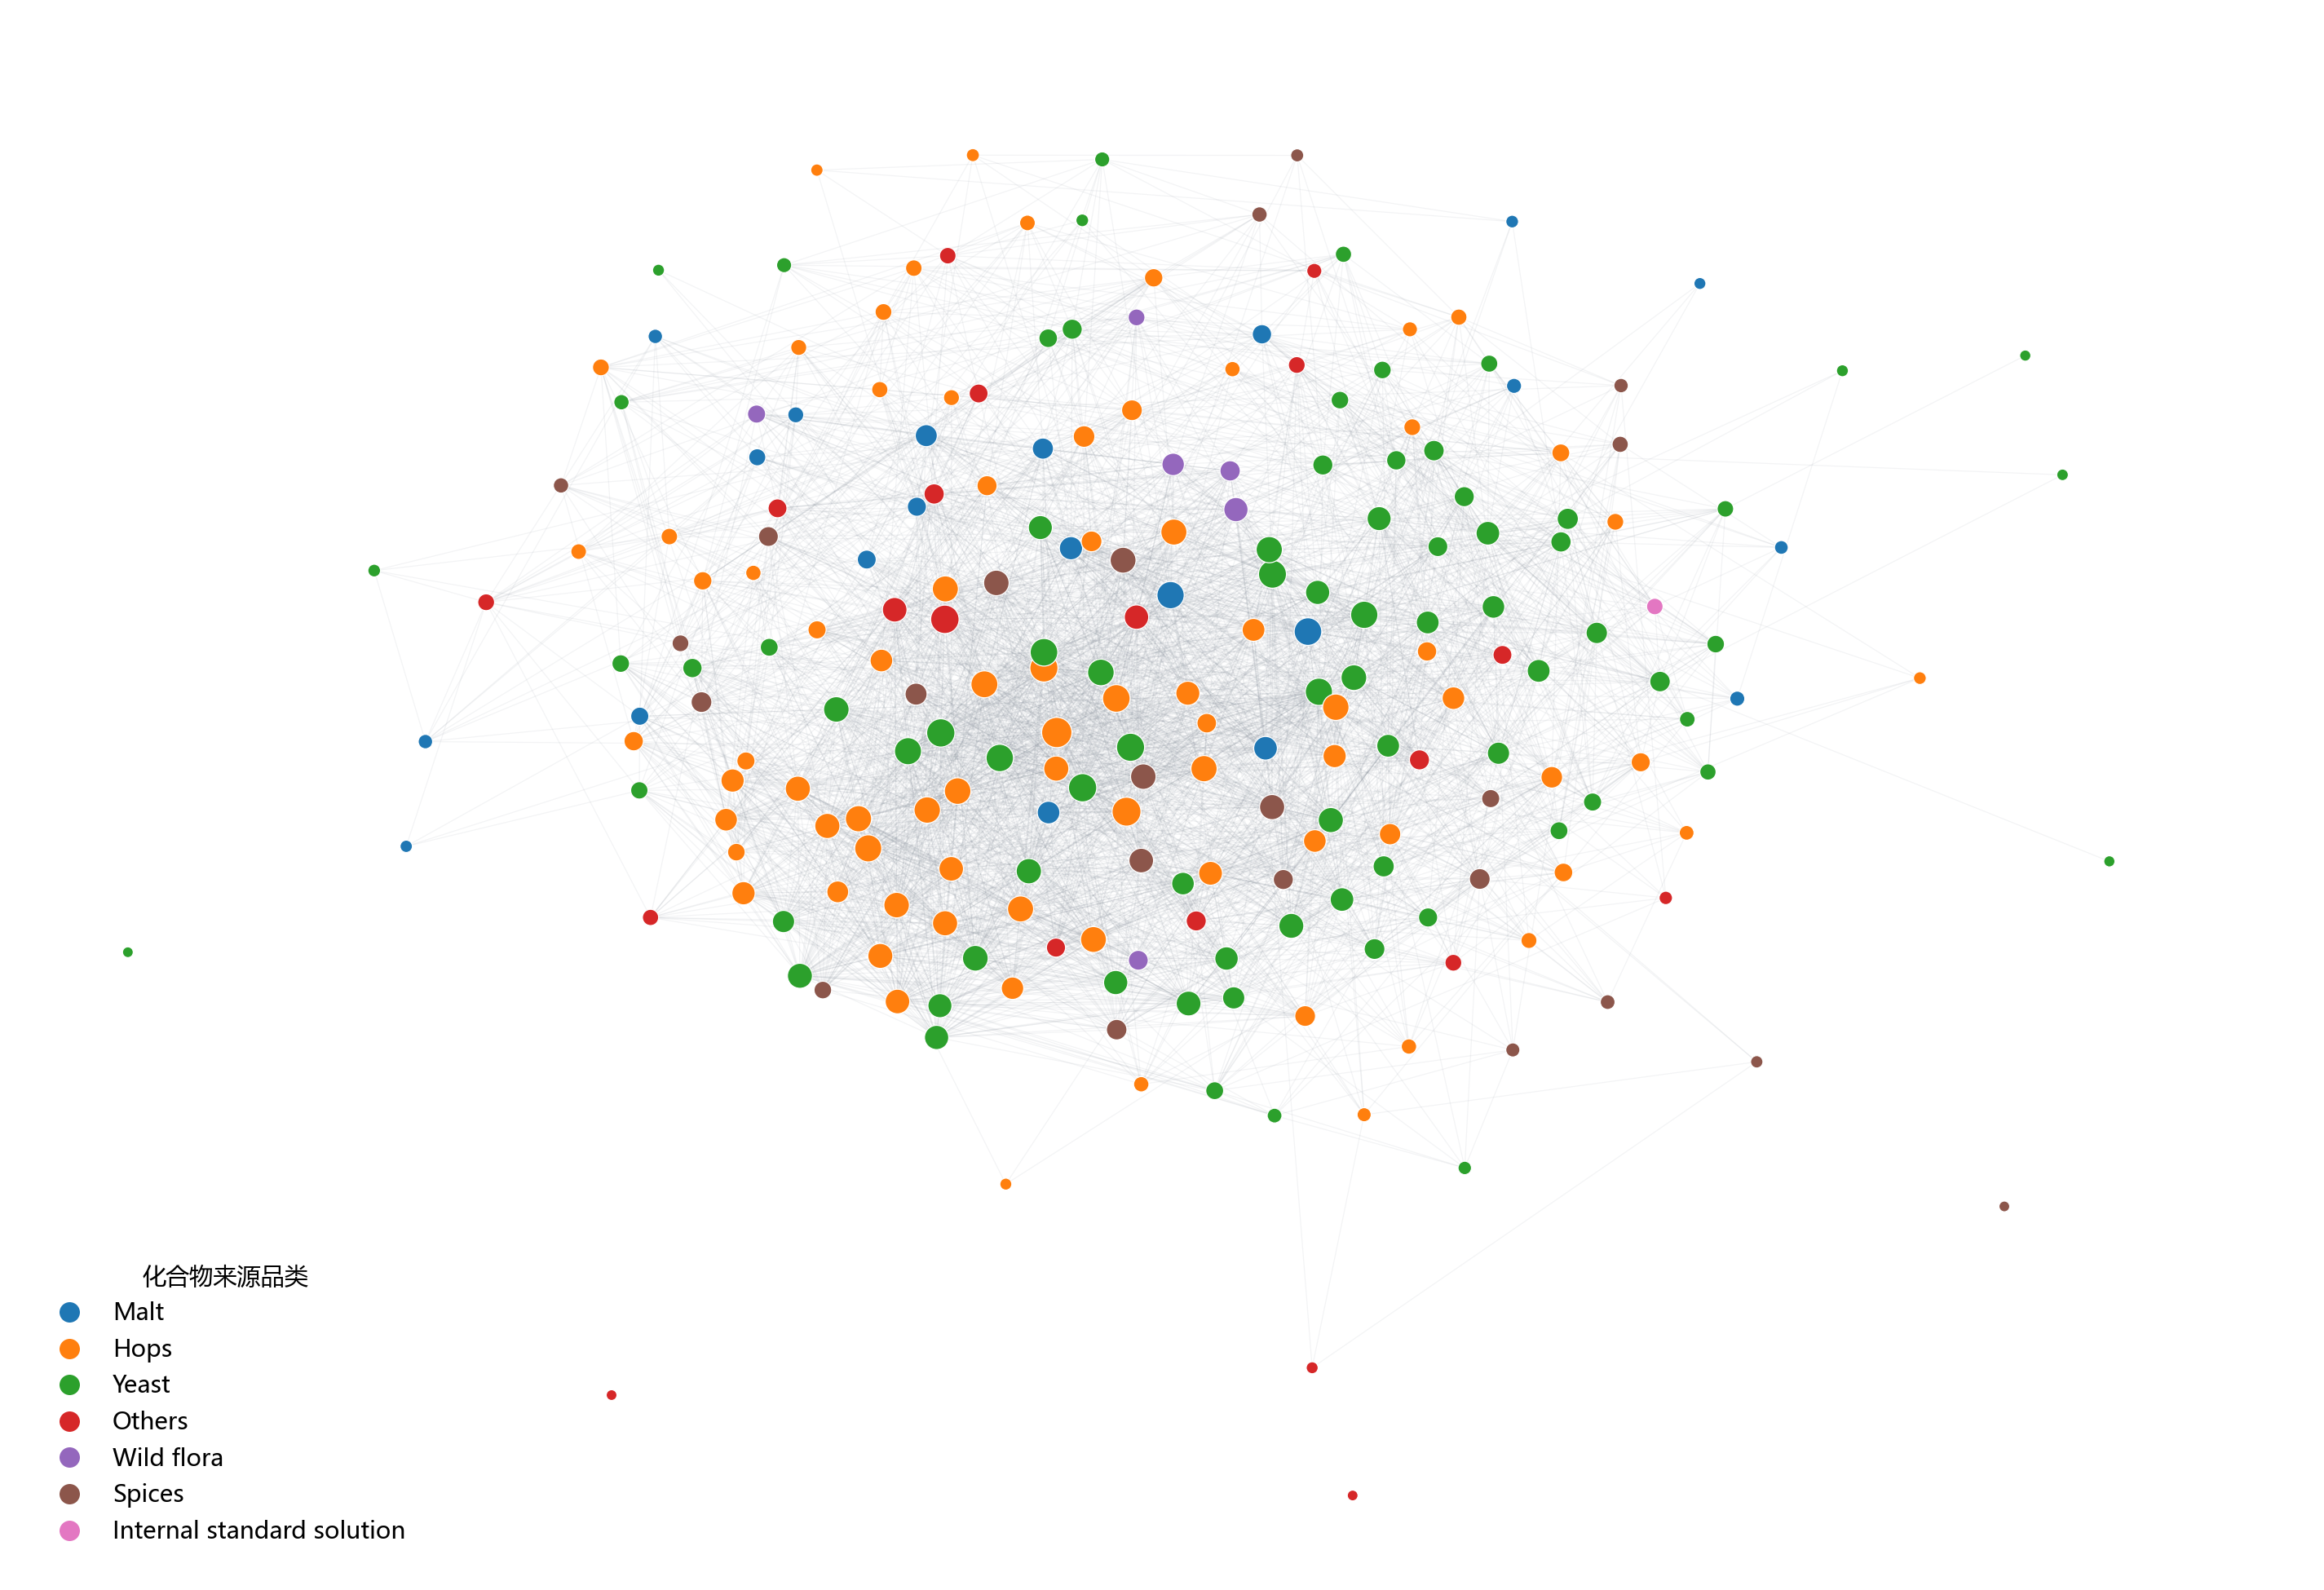
\includegraphics[width=0.88\textwidth]{图M2-01-共表达网络.png}
\caption{化合物共表达网络（边阈值 \textbf{0.30}，边权为 $|\rho|$；节点颜色表示来源品类，节点大小表示连接度）}
\label{fig:q2-network}
\end{figure}

图 \ref{fig:q2-network} 显示网络主体是一个大分量，外围有少量度较低的节点和 \textbf{4} 个孤立点。节点颜色把 Malt、Hops、Yeast、Others、Wild flora、Spices 等来源品类混在一起，说明同一来源的化合物并不总是聚成一团；这也解释了后文品类一致率不可能很高：网络连接由相关结构决定，而不是由来源标签决定。

\subsubsection{Top-3 关键化合物}

表 \ref{tab:q2-top3} 列出 \textbf{8} 个代表性维度的 Top-3 及 bootstrap 入选频率。选择这 \textbf{8} 个维度时，本文兼顾了麦芽、酒花、酯香、酸、苦、醇和整体感七个方向，并保留一个不可比维度 \texttt{overall}，用来看品类核对在缺失品类时的行为。

\begin{table}[H]
\centering
\zihao{-5}
\setlength{\tabcolsep}{4pt}
\begin{tabularx}{\textwidth}{@{}p{0.15\textwidth}p{0.22\textwidth}p{0.22\textwidth}p{0.22\textwidth}p{0.10\textwidth}@{}}
\toprule
感官维度 & 第 \textbf{1} 名（频率） & 第 \textbf{2} 名（频率） & 第 \textbf{3} 名（频率） & 维度品类 \\
\midrule
\texttt{A\_malt\_all} & Color（\textbf{0.975}） & Methylpyrazine（\textbf{0.760}） & Protein（\textbf{0.420}） & Malt \\
\texttt{A\_hops\_citrus} & Citronellol（\textbf{0.625}） & Humulene epoxide II（\textbf{0.290}） & Carbon dioxide（\textbf{0.345}） & Hops \\
\texttt{A\_esters\_ethac} & Ethyl propionate（\textbf{0.760}） & Phenethyl alcohol（\textbf{0.680}） & Acetaldehyde（\textbf{0.320}） & Yeast \\
\texttt{F\_malt\_bread} & Betaglucan（\textbf{0.665}） & Acetaldehyde（\textbf{0.840}） & Isobutanol（\textbf{0.285}） & Malt \\
\texttt{F\_esters\_ethac} & Ethyl propionate（\textbf{0.880}） & Ethyl acetate（\textbf{0.730}） & Acetaldehyde（\textbf{0.420}） & Yeast \\
\texttt{acidity} & Acetic acid（\textbf{0.940}） & pH（\textbf{0.550}） & 4-ethyl-phenol（\textbf{0.425}） & Others \\
\texttt{bitternes} & Iso-alpha acids（\textbf{0.815}） & Ethyl octanoate（\textbf{0.660}） & Dimethyl sulfide（\textbf{0.480}） & Others \\
\texttt{alcohol} & Ethanol（\textbf{1.000}） & Acetaldehyde（\textbf{0.900}） & Isobutanol（\textbf{0.550}） & Yeast \\
\bottomrule
\end{tabularx}
\caption{代表性感官维度的 Top-3 关键化合物与 bootstrap 入选频率}
\label{tab:q2-top3}
\end{table}

表 \ref{tab:q2-top3} 的第 \textbf{1} 名频率普遍高于第 \textbf{3} 名，例如 \texttt{alcohol} 的 Ethanol 为 \textbf{1.000}，\texttt{acidity} 的 Acetic acid 为 \textbf{0.940}，\texttt{F\_esters\_ethac} 的 Ethyl propionate 为 \textbf{0.880}；而 \texttt{A\_hops\_citrus} 的第 \textbf{2} 名只有 \textbf{0.290}，说明该维度的后位排序对样本扰动更敏感。这个差别与后文的整体稳定性结论一致：Top-1 较稳，Top-3 的后两位不稳。

\subsubsection{稳定性}

\textbf{200} 次 bootstrap 的 rank1、rank2、rank3 平均入选频率分别为 \textbf{0.6734}、\textbf{0.4896}、\textbf{0.3611}。在 \textbf{150} 个格子（\textbf{50} 维 $\times$ \textbf{3} 名次）中，频率不低于 \textbf{0.80} 的有 \textbf{22} 格，不低于 \textbf{0.50} 的有 \textbf{72} 格，低于 \textbf{0.50} 的有 \textbf{78} 格，最小值为 \textbf{0.125}。

\begin{figure}[H]
\centering
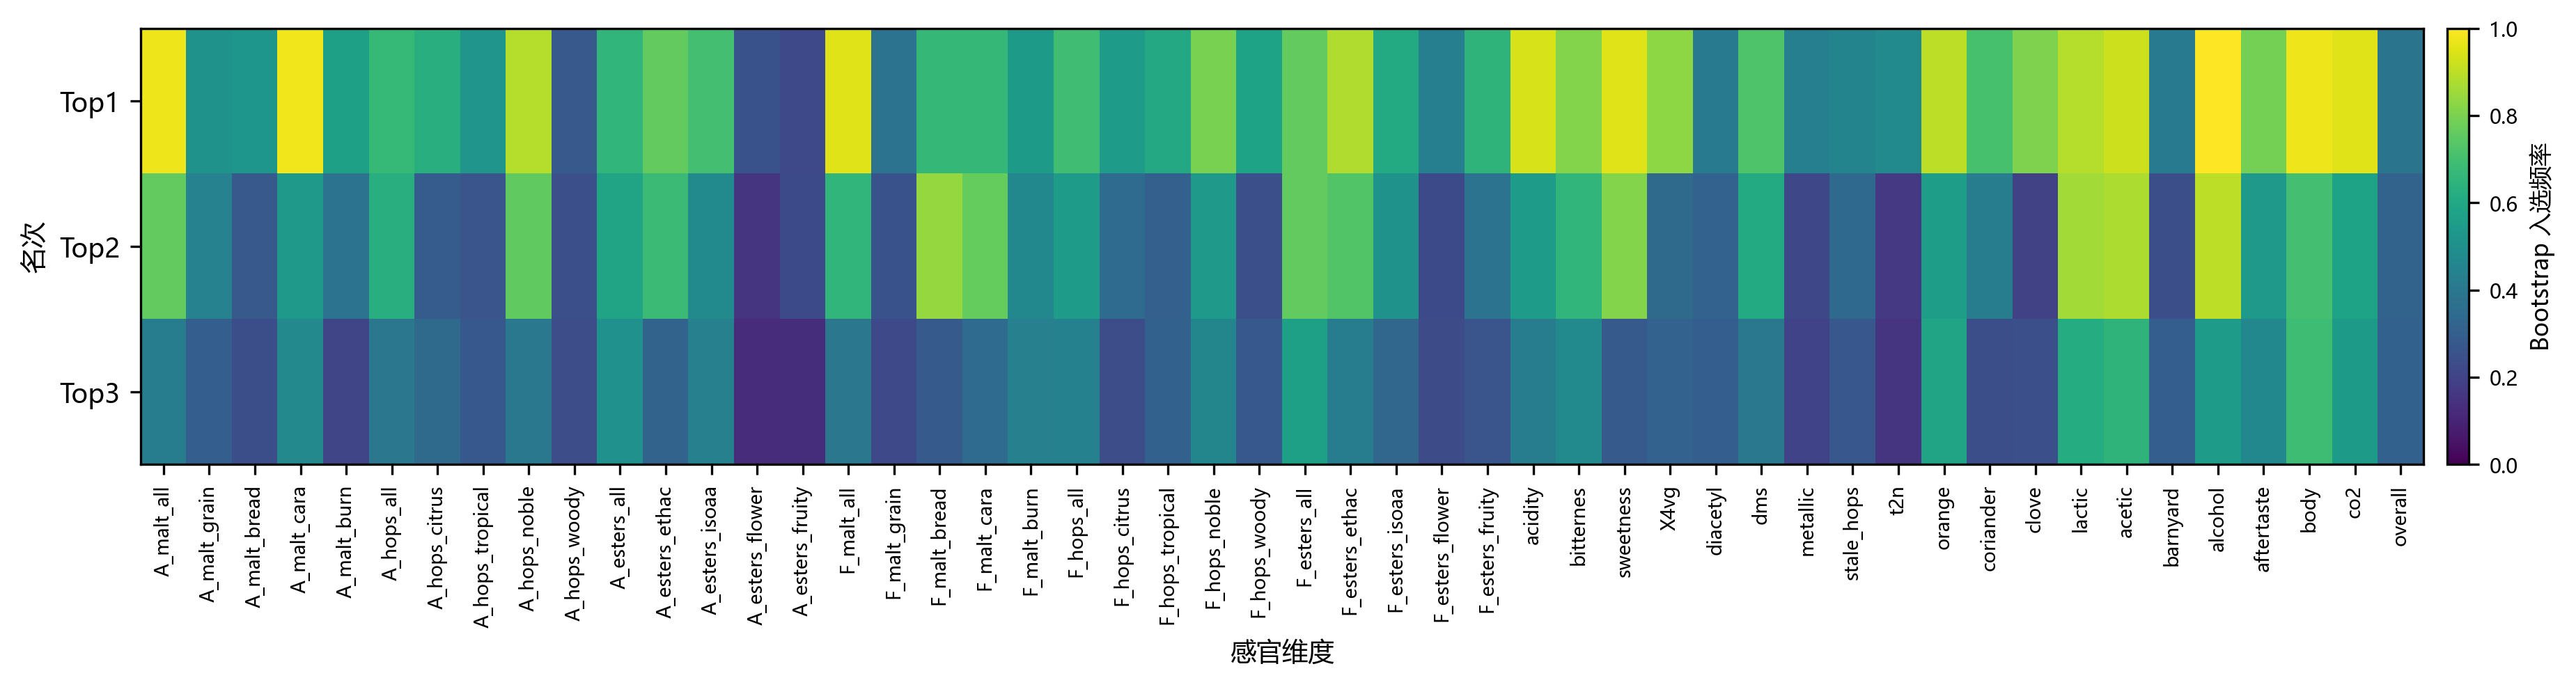
\includegraphics[width=0.98\textwidth]{图M2-02-稳定性频率.png}
\caption{\textbf{50} 个感官维度 Top-3 化合物在 \textbf{200} 次 bootstrap 中的入选频率}
\label{fig:q2-stability}
\end{figure}

图 \ref{fig:q2-stability} 的列是感官维度，行是名次，颜色越亮表示频率越高。亮色主要集中在 Top1 行，Top3 行整体偏暗；这说明“谁是第一”相对稳定，“第三是谁”在很多维度上并不稳定。本文不把这种结果包装成“高度稳定”，也不据此替换 Top-3：频率只用于解释，不用于改排名。若实际应用更看重召回率，可以把 Top-3 当作候选集，再用实验验证后位化合物。

\subsubsection{图项的作用}

$\lambda=0$ 与 $\lambda=0.70$ 的 \textbf{50} 维 Top-3 平均 Jaccard 为 \textbf{0.378}，中位数为 \textbf{0.350}，最小值为 \textbf{0}，最大值为 \textbf{1}。在 \textbf{50} 维中，两种设置重合 \textbf{0} 个、\textbf{1} 个、\textbf{2} 个、\textbf{3} 个的维度分别有 \textbf{3}、\textbf{22}、\textbf{21}、\textbf{4} 个。融合分与直接相关分的跨化合物秩相关均值为 \textbf{0.8693}，最小值为 \textbf{0.8137}；图项得分的跨化合物标准差约为直接相关得分的 \textbf{0.5087} 倍。

\begin{figure}[H]
\centering
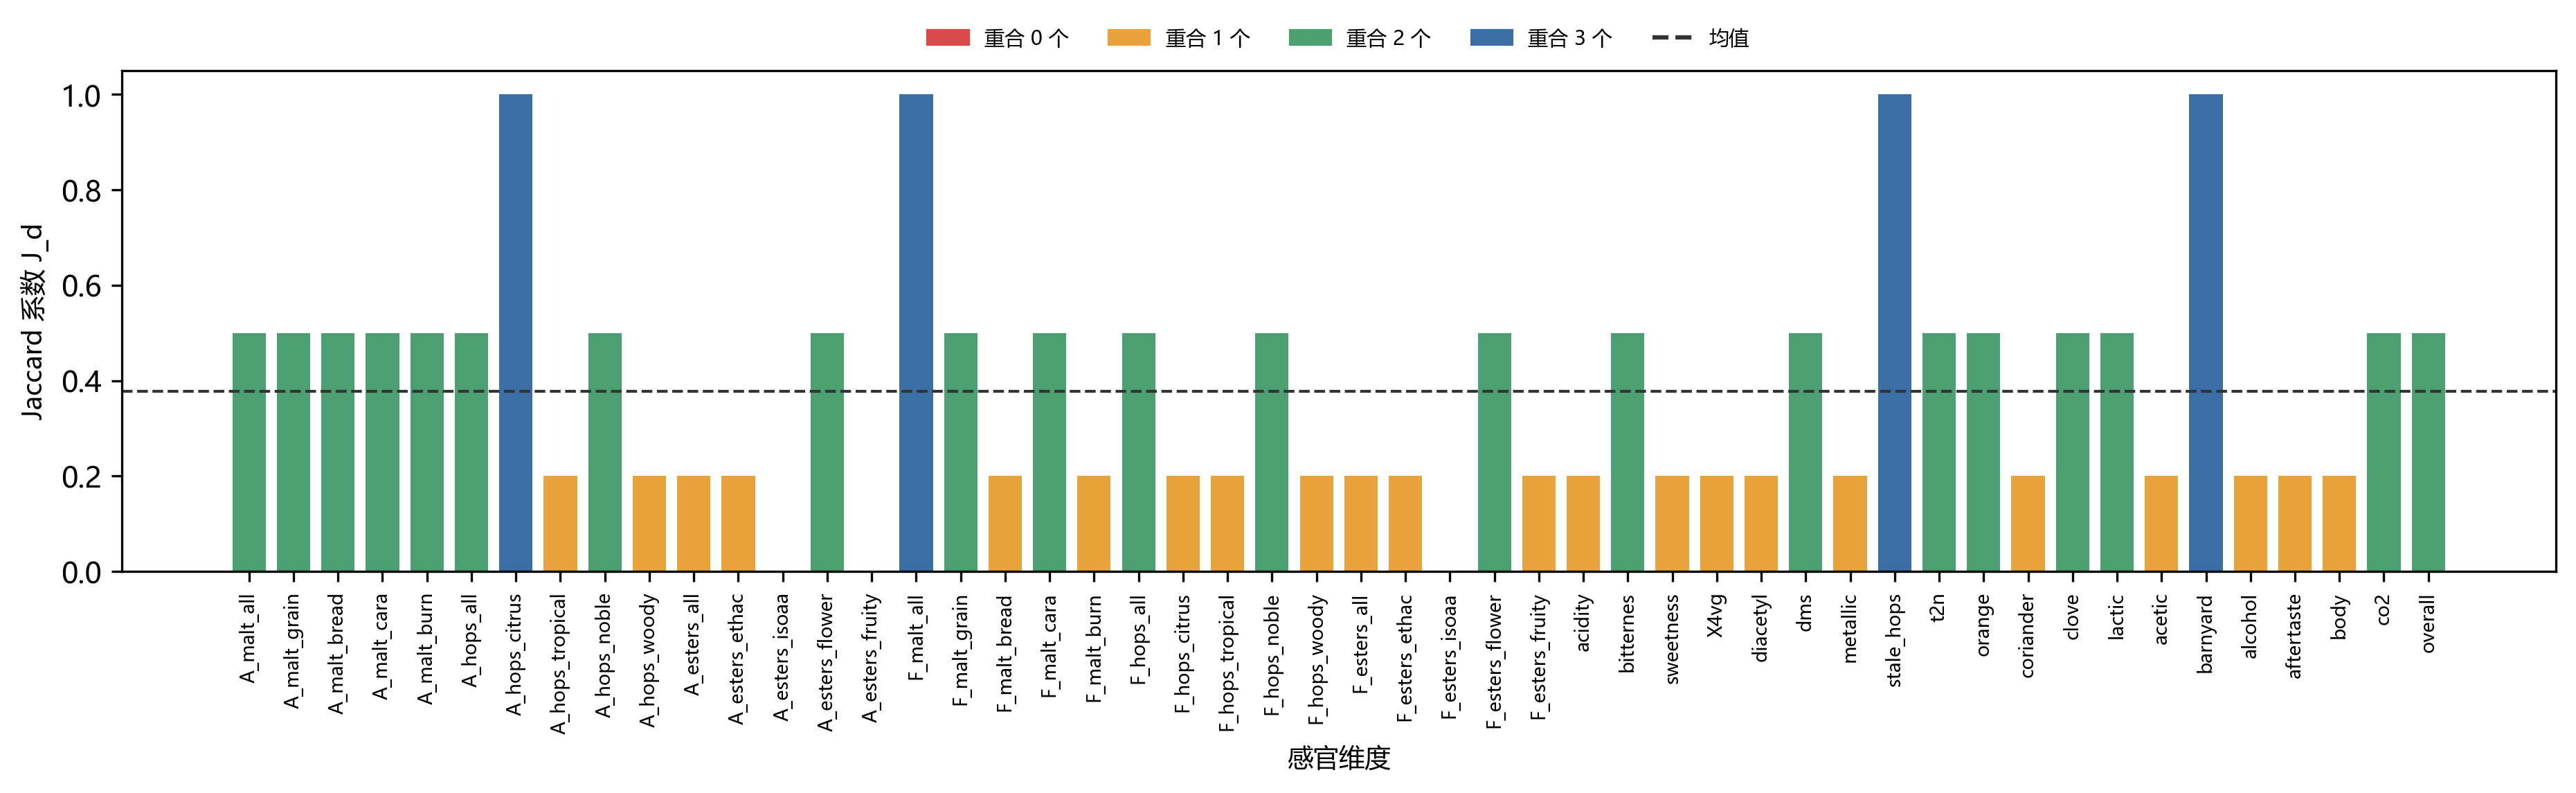
\includegraphics[width=0.98\textwidth]{图M2-03-lambda对照Jaccard.png}
\caption{$\lambda=0$ 与 $\lambda=0.70$ 两种设置下 \textbf{50} 维 Top-3 的逐维 Jaccard 系数}
\label{fig:q2-lambda}
\end{figure}

图 \ref{fig:q2-lambda} 把逐维重合度画成条形图，虚线为 \textbf{50} 维均值 \textbf{0.378}。若图项完全不起作用，所有柱子都应为 \textbf{1}；实际只有 \textbf{4} 维达到 \textbf{1}，多数维度在 \textbf{0.2--0.5} 之间，说明图项确实改变了排序。秩相关 \textbf{0.8693} 又说明融合没有把原排序彻底打乱，图项是在原排序上做局部平滑，而不是另起一套排序。

\subsubsection{化学合理性}

按来源品类核对 \textbf{150} 个 Top-3 格子，一致 \textbf{48} 对、不一致 \textbf{86} 对、不可比 \textbf{16} 对，一致率为 \textbf{0.3582089552}，独立假设基线为 \textbf{0.2047}。不可比的 \textbf{16} 格由两部分组成：\textbf{3} 个缺失品类维度各 \textbf{3} 格，共 \textbf{9} 格；Spices 来源的化合物进入可比维度 \textbf{7} 格。候选池内不可比化合物共 \textbf{24} 个，其中 Spices \textbf{23} 个、Internal standard solution \textbf{1} 个。

这个一致率高于基线，但离半数仍有距离。原因有三：第一，来源品类是粗粒度标签，同一品类下可能包含化学性质差异很大的化合物；第二，Top-3 由相关强度与图平滑决定，不以品类匹配为目标；第三，Spices 与 Internal standard solution 的化合物在感官维度上没有可比的来源品类，只能从分母剔除。若把不可比项强行并入不一致，一致率会被低估；若把它们并入一致，又会高估。本文保留三分类，是为了让分子分母都可复核。

从具体维度看，化学方向是合理的：\texttt{acidity} 的 Acetic acid、\texttt{bitternes} 的 Iso-alpha acids、\texttt{sweetness} 的 Sugars、\texttt{X4vg} 的 4-vinylguaiacol、\texttt{alcohol} 的 Ethanol 都是该感官的已知主要贡献物；\texttt{F\_esters\_ethac} 的 Ethyl propionate 与 Ethyl acetate 属于酯香，\texttt{A\_malt\_all} 的 Color 与 Methylpyrazine 属于麦芽/烘烤方向。与此同时，\texttt{A\_hops\_citrus} 的 Carbon dioxide 与 \texttt{F\_malt\_bread} 的 Betaglucan 更像“相关邻居”而不是直接呈香物，这提示图平滑在带来稳定性的同时，也会引入间接关联。

\subsubsection{GBM 全局对照}

把 \textbf{50} 维 Top-3 合并去重后得到 \textbf{60} 个化合物，它们与 \texttt{8.xlsx} 的 GBM 重要度表交集为 \textbf{60} 个，占选中化合物的 \textbf{100\%}，占 MDI 表的 \textbf{25.974\%}。选中化合物的 MDI 平均分位为 \textbf{0.6201}，\textbf{226} 池的平均分位为 \textbf{0.4971}。

这里必须加一条\textbf{恒真注}：\textbf{60/60} 的重合由“\textbf{226} 候选池是 \textbf{231} 特征子集”这一集合包含关系直接保证，信息量为零，不能把它读成“本文排序与 GBM 重要度一致”。有信息量的是平均分位 \textbf{0.6201} 对 \textbf{0.4971}：它说明本文选中的化合物在 GBM 全局重要度上略高于候选池平均，但差距不大，且 GBM 表没有逐维信息，不能做逐维对照。本文只把它当作全局旁证，不参与 Top-3 的任何计算。

\subsubsection{稳健性检查}

把 $\tau$ 调到 \textbf{0.25} 和 \textbf{0.35}，平均 Jaccard 分别为 \textbf{0.636} 和 \textbf{0.674}；去掉负边只保留正边，平均 Jaccard 为 \textbf{0.648}；把 $\lambda$ 调到 \textbf{0.30} 和 \textbf{0.50}，平均 Jaccard 分别为 \textbf{0.464} 和 \textbf{0.642}。所有扰动下都没有出现“Top-3 完全不变”或“完全改变”的极端，说明主结果对阈值和权重有中等程度的敏感性。

\begin{figure}[H]
\centering
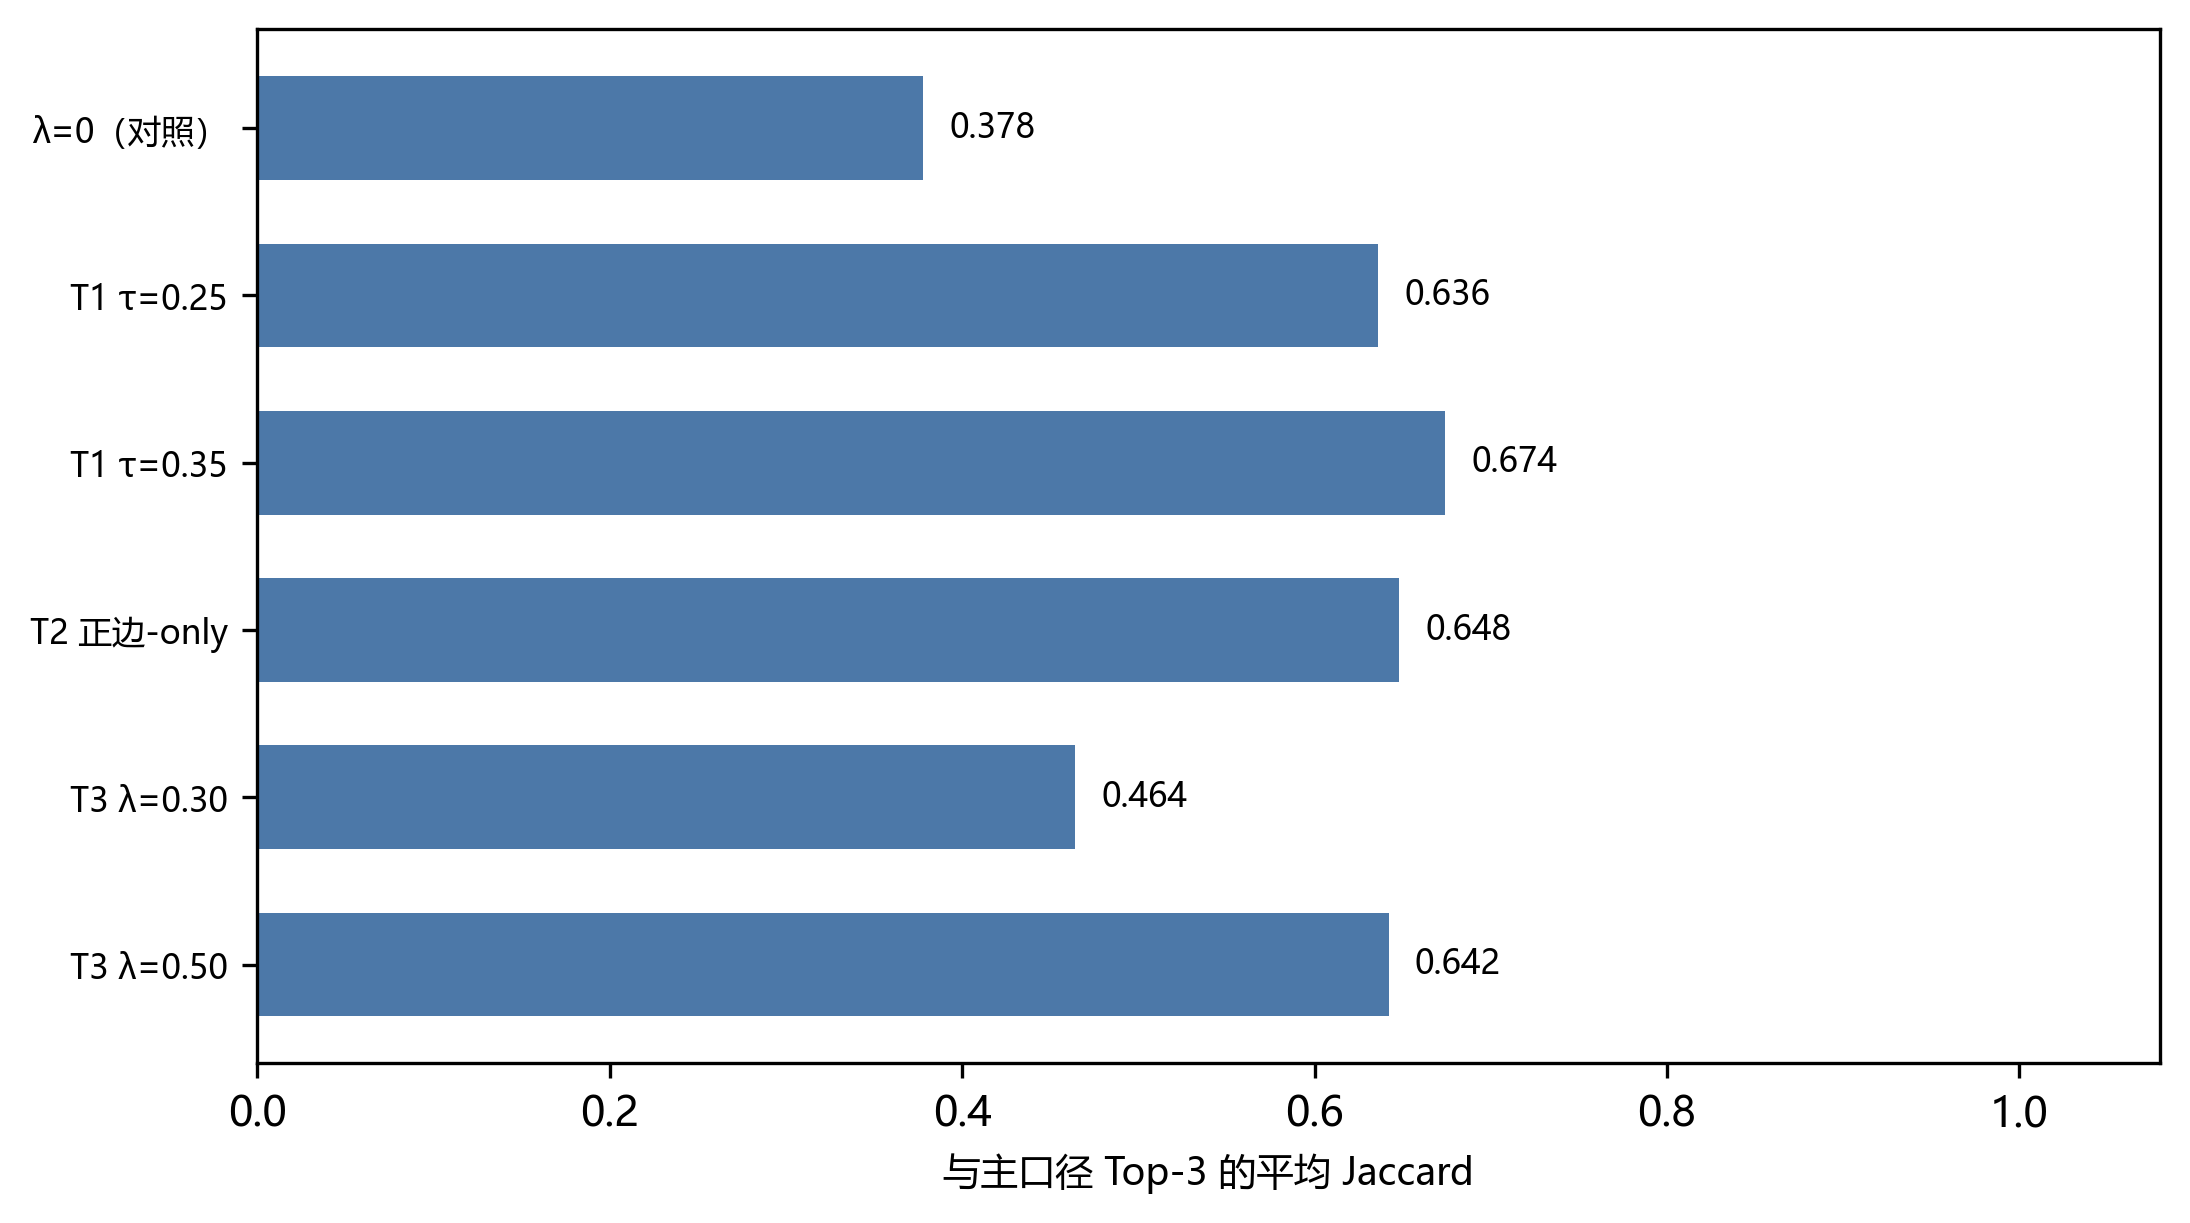
\includegraphics[width=0.82\textwidth]{图M2-04-稳健性检查.png}
\caption{不同图口径与权重设置下 Top-3 与主口径的平均 Jaccard}
\label{fig:q2-robust}
\end{figure}

图 \ref{fig:q2-robust} 中，$\lambda=0.30$ 的 Jaccard 最低（\textbf{0.464}），说明图项权重减半会明显改变后位排序；$\tau=0.35$ 的 Jaccard 最高（\textbf{0.674}），说明把边阈值收紧后，保留的强边足以维持大部分 Top-3。正边-only 的 \textbf{0.648} 说明负边不是排序的主要来源，但去掉负边仍会改变约三分之一的格子，因此负边按绝对值计入是有影响的建模选择，不是可有可无的细节。

\subsubsection{小结}

问题二给出了 \textbf{226} 节点、\textbf{3758} 条边的共表达网络，并用直接相关与图平滑的融合分为每个感官维度选出 Top-3。Top-1 的稳定性高于后两位，图项确实改变了排序，化学方向在多个维度上可解释，但品类一致率只有 \textbf{0.3582}，说明“相关结构上的关键化合物”与“来源品类上的典型化合物”并不是同一个概念。GBM 对照的 \textbf{60/60} 是恒真校验，真正有信息量的是平均分位 \textbf{0.6201} 对 \textbf{0.4971}。这些结果共同支持一个谨慎的结论：本文的 Top-3 可以作为实验验证的候选集，而不宜被当作唯一的因果解释。
